% =========================================================================
% CHAPTER 4
% =========================================================================

\chapter{Protokoll Design}
\label{K4}
Das hier beschriebene Protokoll ist für die Verwendung in einem hierarchischen Client-Server Overlay Network (HCSON) optimiert.
Da in einem solchen Netzwerk Jobs vom Client an den Server und von diesem an Worker gegeben werden, wird im Folgenden zwischen Auftraggeber und Auftragnehmer unterschieden, wobei der Server beide Rollen einnimmt.

Jeder teilnehmende Prozess besitzt eine global eindeutige ID, im Folgenden \NodeID{} genannt, und jeder Job egal ob remote oder nicht, erhält ebenfalls eine ID, im Folgenden \JobID{} genannt.
Alle Messages enthalten eine \JobID{} und beziehen sich jeweils auf genau einen Job.
Zudem enthält jeder Job die \JobID{} des ParentJobs, also jene des Jobs, von dem er erstellt wurde.

Alle Messages sind idempotent. Grundsätzlich entspricht eine Network Message einer State Machine Transition, nur die Return Message repräsentiert die returnOk, returnFail und returnCanceled Transitions. die Return Message enthält ein zusätzliches Flag, das zur Unterscheidung dient.




\section{Network Messages}
\label{messages}

\subsection{\CallMessage{}}
Call Messages werden vom Auftraggeber an den Auftragnehmer gesendet.
Sie enthalten JavaScript Code, der vom Empfänger ausgeführt wird und ersetzen so das Deployment.
Der Enthaltene Code hat seinen Ursprung im \ApplicationLayer{}, er wird beim Erstellen von Jobs definiert (siehe \ref{JobInterface}).

\subsection{\CancelMessage{}}
Cancel Messages werden vom Auftraggeber an den Auftragnehmer gesendet.
Cancel Messages führen nicht unbedingt zum Endzustand Canceled.
Falls der Auftraggeber bereits im Zustand Failed oder Ok ist, wird die Cancel Message ignoriert (siehe \ref{JobInterface}).

\subsection{\UpdateMessage{}}
Update Messages werden vom Auftragnehmer an den Auftraggeber gesendet.
Sie werden ausgelöst durch den Aufruf der \JobUpdate{} Funktion (siehe \ref{JobInterface}).
Update Messages enthalten den vom Auftragnehmer definierten Progress, optional eine für Menschen lesbare Statusinfo, sowie optionale Zwischenergebnise des Aufrufs.

\subsection{\ReturnMessage{}}
Diese Messages werden vom Auftragnehmer an den Auftraggeber gesendet, wenn der Job erfolgreich ausgeführt wurde, eine nicht behandelte Exception aufgetreten oder ein Timeout eingetreten ist.
Dies entspricht den Aufgaben von Futures (siehe \ref{future}, \ref{JobInterface}).
Return Messages können die State Machine Transitions returnOk, returnFail oder returnCanceled auslösen.
Ein Flag in der Message bestimmt die Transition.




\section{Job State Machine}
\label{jfsm}
Ein grundlegendes Problem von Distributed Computing ist es, am Client den Zustand von Remote Calls zu verfolgen.
Acknowledges können auf mehreren Layern zum Einsatz kommen, zum Beispiel nur am Tansport Layer.
In diesem Fall wird meist davon ausgegangen, dass eine erfolgreiche Übertragung auch zu einer erfolgreichen Ausführung führt.
\begin{wrapfigure}{L}{0.25\textwidth}
  \vspace{-20pt}
  \begin{center}
    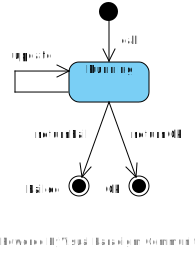
\includegraphics[width=0.25\textwidth]{fsm0}
  \end{center}
  \caption{State Machine eines nicht abbrechbaren RPC}
  \label{fsm0}
\end{wrapfigure}
Algorithmen, bei denen diese Annahme nicht getroffen werden kann, benötigen auch Acknowledges auf dem Application Layer.
Abbildung \ref{fsm0} zeigt eine simple State Machine für einen RPC der nicht abgebrochen werden kann.

An dieser Stelle sollte beachted werden, dass auch diese State Machine verteilt ist.
Sie stellt den Zustand des Remote Calls dar, dieser existiert real am Client und am Server.
Oder mit anderen Worten: Dieser Zustand wird im Stub und im Skeleton gehalten.
Entsprechende Netzwerk Messages synchronisieren den Zustand zwischen Client und Server.
Die \TransReturnOk{} emittiert eine positive \ReturnMessage{}, die \TransReturnFail{} emittiert eine negative \ReturnMessage{}.
Die \TransCall{} wird durch eine \CallMessage{} ausgelöst.

Auch für den Fall, dass kein Abbruch des RPC unterstützt wird und der Server nur am Ende der Ausführung eine Message mit dem Erfolgszustand an den Client sendet, ist es nicht immer möglich, diese State Machines zu synchronisieren. Siehe Zwei-Armeen-Problem \cite{tanenbaum4andrew}.
Denn der Client könnte durch ein Timeout Event, das genau dann eintritt, wenn die Return Message vom Server auf dem Weg zum Client ist, in den Failed Zustand übergehen, während der Server bereits im Ok Zustand ist.

Wird das System so erweitert, dass Remote Calls abgebrochen werden können (siehe Abbildung \ref{fsm1}), trifft man auf dasselbe Problem wenn vom Client eine Abbruch Meldung an den Server gesendet wird und der Server bereits eine Erfolgsmeldung gesendet hat, diese aber noch nicht am Client angekommen ist.
\begin{wrapfigure}{R}{0.45\textwidth}
  \vspace{-20pt}
  \begin{center}
    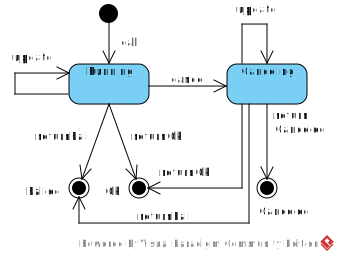
\includegraphics[width=0.45\textwidth]{fsm1}
  \end{center}
  \caption{Erweiterte State Machine eines abbrechbaren RPC}
  \label{fsm1}
\end{wrapfigure}
Eine Strategie um dieses Problem zu minimieren ist es, den Client nicht in den Canceled State übergehen zu lassen ohne vom Server eine Bestätigung erhalten zu haben.
Im Detail bedeutet das, dass der Client in den Canceling State übergeht, eine Nachricht an den Server sendet mit dem Auftrag die Ausführung abzubrechen und dann vom Server den Endzustand erhält.
Soweit scheint es, dass beide am Ende im selben Zustand sind, jedoch muss auch der Canceling State mit einem Timeout überwacht werden, was wiederum zum Zwei-Armeen-Problem führt.

Will man nicht nur am Ende der Ausführung vom Server über dessen Zustand informiert werden, sondern auch während der Ausführung, zum Beispiel über den Progress oder Warnings, so können ebenfalls Race Conditions beim Abbruch auftreten, wenn nicht diese Art der Terminierung verwendet wird.
Der Client könnte durch ein Timeout bereits im Failed State sein, während der Server noch Running States publiziert.

Dabei wird auch offensichtlich, dass Ressourcen verschwendet werden,  während am Client bereits davon ausgegangen wird, dass die Ausführug fehlgeschlagen ist, der Server aber noch daran arbeitet.
In diesem Fall können Ergebnisse nicht vom Client angenommen werden, weil am Client die Ausführung bereits als Fehlerhaft deklariert wurde.

Die Verschwendung dieser Ressourcen kann minimiert werden, in dem der Client im Fall eines Timeouts den Remote Call am Server durch eine Cancel Message beendet
- minimiert deshalb, weil immer noch Netzwerkfehler einen solchen Abbruch verhindern können.
Im Folgenden werden Remote Calls, welche diese State Machine implementieren, Jobs genannt.
Jobs können aber auch rein lokal für asynchrone Aufrufe verwendet werden.
Der das handling von verlorenen Messages ist in diesem Fall zwar nicht notwendig, dennoch können sie hilfreich sein beim auffinden von Implmentierungsfehlern und Race Conditions (siehe Kapitel \ref{K5}).





\section{JobTrees und Call Graphen}
In einem HCSNO ist es üblich Aufgaben zu delegieren. Der Client gibt Aufträge an den Server, der Server an die Worker.
Die einzelnen durchlaufenen Code Stücke können als Directed Acyclic Graph (DAG), der Ahnlichkeiten zu einem lokalen Call Graphen hat, dargestellt werden \cite{yu2005taxonomy}.
Dieser DAG beschreibt den durchlaufenen Workflow über alle Rechner.
In P2P Netzwerken können diese Graphen noch größere Tiefen erreichen.
Jedem Knoten im DAG ist eine Workflow Logic zugeordnet. Typische Workflows sind:
\BCL
  \item Worker werden parallel gestartet und müssen alle erfolgreich terminieren
  \item Worker werden parallel gestartet, einer muss erfolgreich sein (Redundanz)
  \item Worker werden konsekutiv gestartet, alle müssen erfolgreich sein
  \item Pooling. N Worker arbeiten parallel, jedoch gibt es mehr Aufträge als Worker. Schließt ein Worker einen Job ab, beginnt er mit einem der übrigen Jobs, bis alle abgearbeitet wurden
\ECL
Die Vollständigkeit dieser Liste ist nicht gegeben.
Der Anwender muss also die Möglichkeit haben, diese Liste zu erweitern.
Die Javascript Bibliothek async \cite{async} verwendet ein ähnliches Konzept für asynchrone Funktionsaufrufe, und zeigt eine beeindruckende Liste an möglichen Workflows.

Der Workflow DAG dieser Implementierung wird im folgenden JobTree genannt.
Jeder Knoten im JobTree ist eine Job State Machine.
Delegiert ein Job A eine Aufgabe an einen anderen Job B, wird A im folgenden \ParentJob{}, und B \SubJob{} genannt.

Hat ein Knoten in einem Call Graphen mehrere Kinder, bedeutet dies immer sie wurden Konsekutiv ausgeführt.
Im Kontext dieser Arbeit muss es möglich sein Unteraufgaben parallel auszuführen, genauer betrachtet muss es sogar möglich sein den Startzeitpunkt für jede Unteraufgabe frei festzulegen (siehe Pool Workflow).
Die Implementierung des Prototypen verwendet einen Strategy Pattern um den Anwender der Middleware die Möglichkeit zu geben eigene Startsequenzen zu definieren.

Der Zustand des ParentJobs ist von den Zuständen der SubJobs, und der ParentJob Terminate Strategy abhängig.
Die angestrebte Vereinfachung des Middleware APIs  beruht im Wesentlichen darauf, dass die Implementierung des Workflows nicht im Application Layer statt findet, sondern das eine SubJob Start Strategy und eine ParentJob Terminate Strategy aus einer Menge von vordefinierten  Strategien ausgewählt wird.






\begin{wrapfigure}{r}{0.3\textwidth}
  \vspace{-55pt}
  \begin{center}
    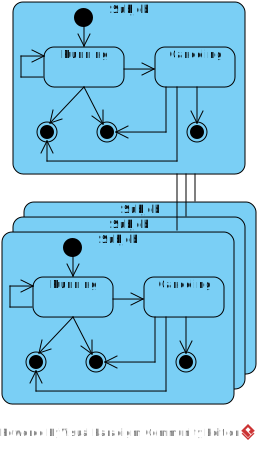
\includegraphics[width=0.3\textwidth]{hfsm}
  \end{center}
  \label{hfsm}
  \caption{Immer wenn eine der untergeordneten State Machines terminiert, wird der Workflow Logic Terminate Strategie aufgerufen.
  Dieser entscheidet ob die Übergeordnete State Machine ihren State ändern muss.}
\end{wrapfigure}
\section{Hierarchische Job State Machine}
Soll ein Job, zum Beispiel am Server, nur die geeigneten Worker ermitteln und die ihm übergebene Aufgabe an diese delegieren, kann die Funktion \JobDelegate{} verwendet werden um dem Job SubJobs hinzuzufügen.
\JobDelegate{} erwartet eine ParentJob Terminate Strategy, eine SubJob Start Strategy, sowie eine Liste der Subjobs.
Anstatt der Liste der SubJobs kann auch eine Factoryfunktion verwendet werden.
\JobDelegate{} bindet Die State Machine des ParentJobs and die der SubJobs, es entsteht eine hierarchische FSM (siehe Abbildung \ref{hfsm}).

Der Aufruf von \JobDelegate{} führt die SubJob Start Strategy aus.
Diese kann nun entscheiden welche SubJobs gleich zu Beginn gestartet werden sollen.
Terminiert ein SubJob wird die ParentJob Terminate Strategy aufgerufen.
Diese muss zunächst entscheiden ob der Parent terminieren soll, wenn nicht kann sie bei bedarf weitere SubJobs starten (siehe Abbildung \ref{seq}).

Wird der ParentJob abgebrochen, wird die \CancelMessage{} an die SubJobs weiter gegeben. Auf Application Layer ist keine Implementierung notwendig.
Terminiert der ParentJob werden et­wa­ige noch laufende SubJobs ebenfalls abgebrochen.
Da bekannt ist wieviele SubJobs vorhanden sind, und welche davon bereits terminiert haben, kann der Progress des ParentJobs bestimmt werden.
Dieses Konzept sollte auch bei P2P Network Overlays anwendbar sein.

JavaScript Promises unterstützen ein ähnliches Konzept.
Promise.race wird für den Fall, dass eine erfolgreiche sub Promise ausreichend ist verwendet und Promise.all für den Fall, dass die erfolgreiche Ausführung aller sub Promises obligat ist.

\begin{wrapfigure}{R}{1\textwidth}
  \vspace{-20pt}
  \begin{center}
    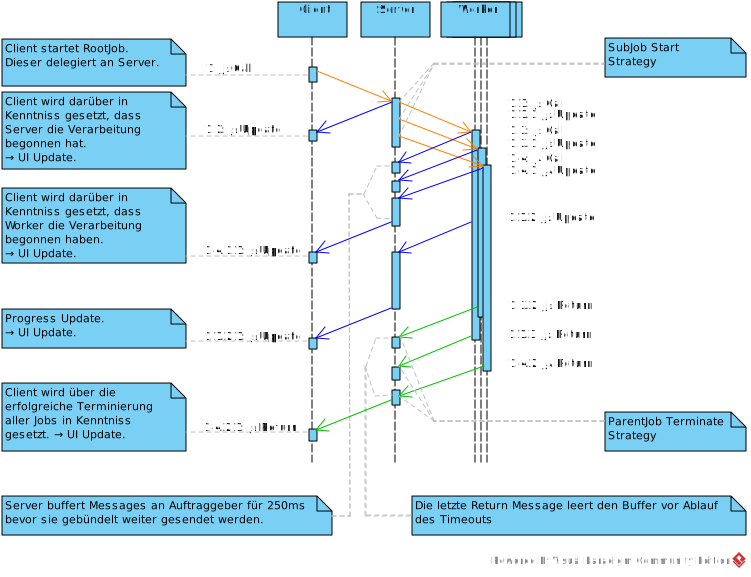
\includegraphics[width=1\textwidth]{seq}
  \end{center}
  \caption{UML Sequenz Diagramm eines Parallel Workflows. Einfachster Fall ohne Fail oder Cancel Messages.PartentJob terminiert wenn alle SubJobs terminiert haben. $J_1$ ist RootJob, und zugleich ParentJob von $J_2$, $J_3$ und $J_4$. Orange sind Call Messages, Blau Update Messages und Grün ReturnOk Messages.}
  \label{seq}
\end{wrapfigure}
